% arara: pdflatex: { synctex: yes }
% arara: makeindex
% arara: pdflatex

\documentclass[12pt,a4paper,twoside]{article}
\usepackage[utf8]{inputenc}

\usepackage{graphicx}
\usepackage{gchords}
\usepackage{guitar}

\usepackage{multicol}
\usepackage{makeidx}
\usepackage[columns=3]{idxlayout}
\usepackage{tocloft}
\usepackage[linktocpage=true]{hyperref}

\usepackage{perpage}

\newcounter{NoS} % number of songs counter
\newcommand{\newsong}[2]
{
	\section{#1}
	\index{#1} 
	\stepcounter{NoS}
	\hfill {\footnotesize#2}
%	\large
}

\newcommand*\cleartoleftpage{%
	\clearpage
	\ifodd\value{page}\hbox{}\newpage\fi
}

\usepackage{titlesec}
\titlespacing*{\section}{0pt}{-3ex}{-3ex}

%\def\guitarEndLine{\par\leavevmode}
%\renewcommand{\guitarEndLine}{\par}
\setlength{\parindent}{0pt}
\setlength{\parskip}{-10pt}
\renewcommand{\baselinestretch}{0.8}

%\author{Pavel Mačák}
\makeindex
\AtBeginDocument{\renewcommand\indexname{Obsah}}

\newcounter{songGroup}
\AddAbsoluteCounter{page}
\newcommand{\includesongs}[1]{
	\stepcounter{songGroup}
	\setcounter{page}{1}
	\renewcommand{\thepage}{\Roman{songGroup}-\arabic{page}} %-\arabic{abspage}
	\include{#1/#1}
}

\newcommand{\slpc}{\vfill\null\columnbreak} % new column
\renewcommand{\familydefault}{\sfdefault}

\renewcommand\guitarPreAccord{\bf\Large\strut}

\renewcommand{\baselinestretch}{1.5}  %individually {\setstretch{1.0} ........... }

\renewcommand{\cftsecleader}{\cftdotfill{\cftdotsep}}

\usepackage{ragged2e}
\newenvironment{raggedmulticols}[1]{%
	\RaggedRight
	\begin{multicols}{#1}%
	}{%
	\end{multicols}%
}


\usepackage[a4paper,
inner=10mm,
outer=10mm,% = marginparsep + marginparwidth 
%   + 5mm (between marginpar and page border)
top=10mm,
bottom=20mm,
marginparsep=5mm,
marginparwidth=40mm,
%showframe% for show your page design, normaly not used
]{geometry}




%%adding chords
%\smallchords
%\def\numfrets{5}
%\begin{minipage}[c]{\linewidth} % use less space
%
%\chords{
%\chord{t}{n,p3,p2,n,p1,n}{C}
%\chord{t}{p3,p2,n,n,n,p3}{G}
%\chord{t}{n,p3,p2,p3,p1,n}{C7}
%\chord{t}{n,n,n,p2,p3,p2}{D}
%\chord{t1}{n,p2,p2,p1,n,n}{F}
%}
%\end{minipage}



\setcounter{secnumdepth}{-2}
\renewcommand{\contentsname}{Obsah}
\renewcommand{\thepage}{ }

\begin{document}
\title{	
	\vspace{3cm}
	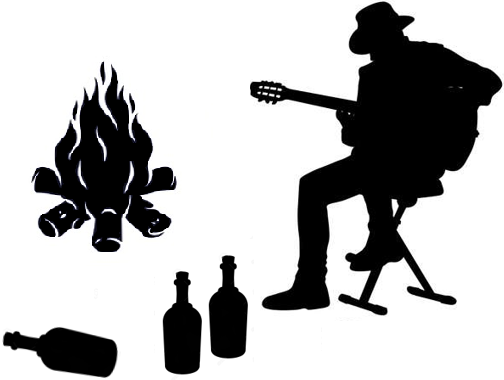
\includegraphics[width=0.75\linewidth]{figs/title_cropped.png}
	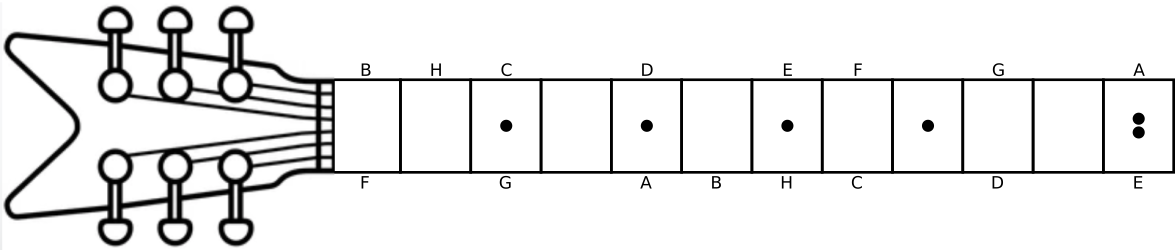
\includegraphics[width=1\linewidth]{figs/stupnice.png}
	
	Zpěvník
}
\date{\today
	\vspace{3.3cm}
	\hfill 
\includegraphics[width=4cm]{figs/qrcode_print-newest.png}}

\maketitle

\newpage

%\begin{multicols}{3}
%	\tableofcontents
%\end{multicols}

\printindex
\newpage

% -------

\includesongs{_adrz}
\includesongs{Kryl}
\includesongs{Nohavica}
\includesongs{Chinaski}
\includesongs{Kabat}
\includesongs{Traband}
\includesongs{Vypsana_fixa}
\includesongs{Zavis}
\includesongs{English}
% --------


\begin{multicols}{2}
	
	\newsong{Mravenčí ukolébavka}{Svěrák a Uhlíř}
	\begin{guitar}
		%!TEX ROOT=../zpevnik.tex

[C]Slunce šlo [G]spát 
[F]za hromádku [G]klád
[C]na nebi [Am]hvězdy klí[G]\null čí.
[C]Už nepra[G]cuj, [F]mravenečku [G]můj,
[C]schovej se [G]do jehli[C]\null čí.


[C]Máš [F]nožičky [C]uběha[G]né,
[C]den [F]byl tak tě[G]\null žký.
[C]Pojď, [F]lůžko máš [C]odestla[G]né
[C]v chládku [F]od maceš[C]ky.

\slpc

Spinká a sní
mravenec lesní
v hromádce u kapradí.
Nespinká sám,
s maminkou je tam,
tykadlama ho hladí.

Máš nožičky uběhané,
den byl tak těžký.
Pojď, lůžko máš odestlané
v chládku od macešky.
	\end{guitar}

\end{multicols}
\bigskip
% --------

Celkem písniček: (\arabic{NoS})
\end{document}
